
This layer is responsible for binding all modules of the Turing Board into one cohesive system. All data coming in is intercepted by this layer and forwarded to the respective modules, which are responsible for processing the forwarded data.

\subsection{Data Processing}
There are three main components of the project which requires this piece of software and must all be non-blocking in nature to ensure the entire system stays responsive.
\begin{itemize}
    \item Reading data from the micro-controller.
    \item Forwarding data to the micro-controller.
    \item Fetching data from the Firebase Real-time database.
\end{itemize}

\begin{figure}[h!]
	\centering
 	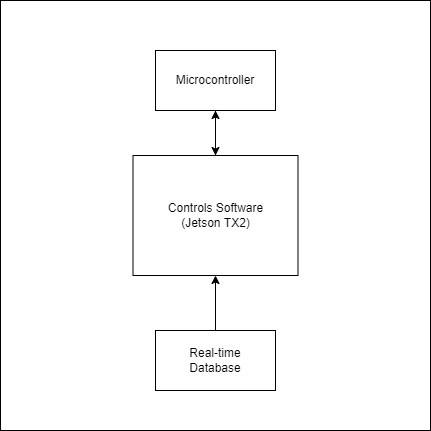
\includegraphics[width=0.60\textwidth]{images/Controls Software Subsystem.drawio.png}
 \caption{Example subsystem description diagram}
\end{figure}

\subsubsection{Assumptions}
The user of the Turing Board is assumed to always be connected to a network (and access the World Wide Web) to ensure data can be received from the database and forwarded to the wheels.

\subsubsection{Responsibilities}
After fetching data from the database, the controls software will first process the data to an extent. Since incoming data will be floating point values, it first needs to be translated into a value which the micro-controller can understand. Thus, the entire range of data is relayed from the remote control app and the required data is then mapped from 0-255, which is then forwarded to the micro-controller. This, in turn, causes the wheels to change speed as needed. As part of the same data packet, angle data from the controls code is also sent to the micro-controller, which aids in rotating the turning mechanism to a specific angle with respect to the origin (0 degrees). Any data, such as weight values for someone who is standing on the longboard (an integral part of the design so that the software knows when to turn off the turning mechanism) is received back in the same data format (0-255), which then gets translated to weight values inside of the controls code.

\subsubsection{Subsystem Interfaces}
Each of the inputs and outputs for the subsystem are defined here.

\begin {table}[H]
\caption {Controls Software Interfaces} 
\begin{center}
    \begin{tabular}{ | p{1cm} | p{5cm} | p{3cm} | p{5cm} |}
    \hline
    ID & Description & Inputs & Outputs \\ \hline
    \#1 & Data Fetching \& Wheel Velocity Control & \pbox{3cm}{Speed Value} & \pbox{5cm}{Change Wheel Velocity}  \\ \hline
    \#2 & Controlling Turning Mechanism & \pbox{3cm}{Angle Value \\ Weight Value} & \pbox{5cm}{Rotates the Turning Mechanism \\ Toggles Turning Mechanism (On/Off)}  \\ \hline
    \end{tabular}
\end{center}
\end{table}
